\documentclass[11pt]{article}

\usepackage[margin=1in]{geometry}
\usepackage{amsmath,amssymb,amsthm,mathtools}
\usepackage{booktabs,array,multirow}
\usepackage{hyperref}
\usepackage{tikz}
\usepackage{pgfplots}
\usepackage{enumitem}
\usepackage{caption}
\usepackage{subcaption}
\usepackage{xcolor}
\usepackage{microtype}
\pgfplotsset{compat=1.18}
\usetikzlibrary{arrows.meta,positioning,calc,fit,shapes.geometric,shapes.misc,backgrounds,decorations.pathreplacing,patterns,intersections}

\hypersetup{colorlinks=true, linkcolor=blue!45!black, citecolor=blue!45!black, urlcolor=blue!45!black}
\setlist[itemize]{leftmargin=1.2em}
\setlist[enumerate]{leftmargin=1.5em}

\newtheorem{definition}{Definition}[section]
\newtheorem{assumption}{Assumption}[section]
\newtheorem{theorem}{Theorem}[section]
\newtheorem{proposition}{Proposition}[section]
\newtheorem{corollary}{Corollary}[section]
\newtheorem{remark}{Remark}[section]

\newcommand{\KP}{K_P}
\newcommand{\KB}{K_B}
\newcommand{\KC}{K_C}
\newcommand{\Xstar}{X^{\ast}}
\newcommand{\A}{\mathcal{A}}
\newcommand{\D}{\mathcal{D}}
\newcommand{\Ccorr}{\mathcal{C}}
\newcommand{\R}{\mathcal{R}}
\newcommand{\F}{\mathcal{F}}
\newcommand{\E}{\mathbb{E}}
\newcommand{\Prob}{\mathbb{P}}
\newcommand{\eps}{\varepsilon}

\title{\textbf{Alignment as a Dynamical System Under Incomplete Constraint Representation}\\
\large Scaling Laws, Viable Regions, and the Geometry of Divergence}

\author{Armando Sori\\
Independent Researcher\\
\texttt{research@simulateai.io}}
\date{April 2026}

\begin{document}
\maketitle

\begin{abstract}
Systems often improve on internal objectives while drifting away from the realities they are intended to serve. This pattern appears in artificial intelligence, digital platforms, economic systems, and institutions. We propose a general theory of alignment for optimizing systems operating under incomplete representations of layered constraints. Alignment is defined as the probability mass of a system trajectory distribution that remains within a viable region of state space. The viable region is induced by physical or feasibility constraints, biological or human-impact constraints, constructed or task-level constraints, and feedback constraints governing what the system can observe.

The paper derives a compact alignment dynamics equation in which alignment changes according to the balance between optimization pressure, constraint misclassification, feedback fidelity, irreversible loss, correction capacity, and viable-region drift. From this formulation we state three named results. The Alignment Incompleteness Law shows that finite representations induce irreducible alignment-estimation error. The Alignment Scaling Law shows that, when misclassification is nonzero and feedback is incomplete, increasing optimization pressure amplifies divergence unless correction scales proportionally. The Viable Design Space Theorem shows that optimization can expand the reachable set while contracting the stable subset of viable designs. We then give a reviewer-facing experimental design and a small real-output pilot illustrating the predicted capability-alignment divergence and its reduction under correction-oriented prompting.

The central implication is a reframing: alignment is not a static property achieved once through objective specification, reward design, or verification. Alignment is a dynamical condition maintained only when systems continue to detect, correct, and recover faster than they drift. The correct design target is therefore not perfect alignment, but stable alignment under unavoidable representation error.
\end{abstract}

\tableofcontents
\newpage

\section{Introduction}

Modern optimizing systems frequently exhibit a gap between visible performance and real-world validity. Language models become more fluent while still hallucinating. Digital platforms become better at maximizing engagement while degrading informational quality. Economic systems improve short-run output while externalizing ecological and social costs. Institutions optimize internal scorecards while drifting from public mission. These cases are usually studied separately. This paper advances a different claim: they are instances of a common dynamical structure.

The proposed structure is optimization under incomplete constraint representation. Systems do not act directly on the full state of the world. They act through internal models, proxy objectives, feedback signals, metrics, and partial observations. If those representations omit, misclassify, or weakly observe constraints that matter for viability, increasing optimization pressure can make the system better at exploiting what it represents while making it worse relative to the full constraint structure that determines whether its behavior is actually viable.

This paper develops that claim as a formal alignment theory. We model reality as a layered constraint structure
\[
\R = (\KP,\KB,\KC),
\]
where \(\KP\) denotes physical, factual, material, or feasibility constraints; \(\KB\) denotes biological, human-impact, cognitive, or social-viability constraints; and \(\KC\) denotes constructed, institutional, policy, task-level, or metric constraints. The labels are intentionally portable. In an AI system, \(\KP\) may include factual truth, numerical validity, and physical feasibility; \(\KB\) may include safety, human impact, cognitive load, and uncertainty calibration; and \(\KC\) may include format, instruction adherence, benchmarks, or policy. In an economy, \(\KP\) may include thermodynamic, ecological, and resource constraints; \(\KB\) may include health, stress, trust, and social cohesion; and \(\KC\) may include money, law, accounting, prices, contracts, and institutions.

The contribution of the paper is not to collapse all domains into one scalar metric. The contribution is to identify a shared geometry of failure and a shared logic of stability. When reward hacking, hallucination, Goodhart effects, delayed externalities, institutional drift, hidden fragility, and overshoot appear in different domains, they often share the same deeper mechanism: optimization over a partial representation of a constrained world.

\subsection{Core claim}

The core claim can be written informally as follows:
\begin{quote}
A system remains aligned only if its correction capacity scales at least as fast as pressure-amplified misclassification under incomplete feedback.
\end{quote}

Formally, let \(A(S,t)\in[0,1]\) denote alignment at time \(t\). We model alignment dynamics as
\begin{equation}
\frac{dA}{dt} = -\pi\eps(1-\gamma) - \Lambda + C - \Phi,
\label{eq:alignment-dynamics}
\end{equation}
where \(\pi\) is optimization pressure, \(\eps\) is misclassification error, \(\gamma\in[0,1]\) is feedback fidelity, \(\Lambda\) is irreversible loss, \(C\) is correction capacity, and \(\Phi\) is viable-region drift. This is not proposed as a literal physical law. It is a compact systems model that makes the relevant levers explicit.

\subsection{Contributions}

The paper makes six contributions.

\begin{enumerate}
    \item \textbf{Layered constraint ontology.} We define alignment over a viable region induced by physical, biological, constructed, and feedback constraints rather than over a single objective.
    \item \textbf{Dynamic alignment equation.} We express alignment change as a balance between divergence pressure and correction capacity.
    \item \textbf{Three named results.} We state the Alignment Incompleteness Law, Alignment Scaling Law, and Correction Scaling Law as implications of incomplete representation and finite correction.
    \item \textbf{Viable Design Space Theorem.} We show that increasing optimization pressure can expand reachability while contracting stable viability.
    \item \textbf{Capability-alignment divergence experiment.} We define an empirical signature: \(\Delta = \mathrm{Capability} - \mathrm{Alignment}\), and give a falsifiable experiment using pressure and correction interventions.
    \item \textbf{Native TikZ visualization package.} All figures in this paper are implemented directly in \LaTeX{} using TikZ/PGFPlots for arXiv portability.
\end{enumerate}

\subsection{Reviewer-facing scope}

The paper is deliberately conservative about what it proves. It does not prove that all systems must fail, that capability is harmful, or that one metric can resolve all normative disputes. It argues that under finite representation, nonzero misclassification, incomplete feedback, and increasing pressure, alignment is not guaranteed by objective specification alone. It must be maintained dynamically.

\section{Related Work}

\paragraph{Goodhart effects and proxy optimization.} Goodhart's Law states that measures lose validity when optimized as targets \cite{goodhart1975problems}. Later taxonomies distinguish multiple failure modes, including regressional, extremal, causal, and adversarial Goodhart effects \cite{manheim2019categorizing}. The present framework embeds Goodhart effects inside a layered constraint ontology: metrics fail not merely because they are optimized, but because the metric is an incomplete representation of a deeper constraint field.

\paragraph{AI alignment and reward misspecification.} AI safety research has emphasized reward hacking, negative side effects, distribution shift, robustness failures, and specification gaming \cite{amodei2016concrete}. Reinforcement learning formalizes optimization over reward signals \cite{sutton2018reinforcement}; when reward is incomplete, the optimized behavior may diverge from intended outcomes. RLHF and reward modeling improve many aspects of assistant behavior but still operate through learned proxies \cite{leike2018scalable,bai2022training}. Truthfulness benchmarks reveal that models can produce confident falsehoods and imitate common misconceptions \cite{lin2022truthfulqa}. This paper generalizes those concerns into a dynamical relation between pressure, feedback, correction, and viable state space.

\paragraph{Control theory and stability.} Control theory provides a vocabulary for stability, feedback, bounded disturbance, and correction \cite{khalil2002nonlinear}. The present theory borrows that logic but differs from classical control formulations in two ways. First, the viable region may be only partially observable. Second, the viable region itself may drift over time as environments, populations, or system effects change.

\paragraph{Institutions, ecology, and commons.} Institutional and ecological theory emphasize externalities, delayed costs, commons failure, legitimacy, and irreversibility \cite{ostrom1990governing}. These are natural examples of layered misalignment: constructed systems can delay or redistribute contact with lower-layer constraints, but cannot repeal them. When feedback is slow or distorted, systems may appear successful internally while accumulating real external burden.

\paragraph{Contribution relative to prior work.} The paper's contribution is not a replacement for domain-specific theories. It is a unification layer. It gives a common language for describing why a reward function, market price, institutional metric, or platform engagement signal can improve while validity degrades.

\section{Layered Constraint Ontology}

\begin{definition}[Layered constraint structure]
Let \(X\) be a system state or output space. A layered constraint structure is a tuple
\[
\R = (\KP,\KB,\KC),
\]
where \(\KP,\KB,\KC\subseteq X\) represent feasibility, human-impact, and constructed constraints respectively.
\end{definition}

\begin{definition}[Viable region]
The viable region is a subset
\[
\Xstar(\omega,\tau,\alpha,t) \subseteq X,
\]
parameterized by reference population \(\omega\), time horizon \(\tau\), aggregation rule \(\alpha\), and time \(t\). A simplified constraint-intersection form is
\[
\Xstar(t) = \KP(t)\cap\KB(t)\cap\KC(t).
\]
\end{definition}

\begin{remark}[Contested edges]
The notation \(\Xstar(\omega,\tau,\alpha,t)\) makes explicit that viability is not always a neutral scalar. Different populations, time horizons, and aggregation rules can induce different viable regions. The framework allows contested alignment at the edges while preserving the possibility of a minimal floor of states that are broadly inadmissible.
\end{remark}

\begin{definition}[Floor viable set]
Let \(\Omega\) be a set of admissible reference populations, \(T\) a set of admissible horizons, and \(\mathcal{G}\) a set of admissible aggregation rules. The floor viable set is
\[
\Xstar_{\mathrm{floor}}(t) = \bigcap_{\omega\in\Omega,\tau\in T,\alpha\in\mathcal{G}} \Xstar(\omega,\tau,\alpha,t).
\]
\end{definition}

The floor set is typically small. Its role is not to resolve all normative disagreement, but to distinguish bounded contestation from catastrophic collapse.

\subsection{Biological constraints are not monolithic}

Earlier formulations of layered alignment can be too simple if they treat \(\KB\) as one coherent block. Biological and human-impact constraints often conflict: short-term reward versus long-term survival, individual advantage versus collective stability, autonomy versus attachment, exploration versus safety, and speed versus deliberation.

\begin{definition}[Biological constraint topology]
Let
\[
\mathcal{B}=\{B_1,B_2,\ldots,B_m\}
\]
be a set of biological or human-impact constraint clusters. Each cluster \(B_i\) represents a coherent class of demands, such as safety, belonging, cognition, status, health, or long-horizon planning.
\end{definition}

\begin{definition}[Conflict relation]
A conflict relation \(\Gamma\subseteq\mathcal{B}\times\mathcal{B}\) is defined by
\[
(B_i,B_j)\in\Gamma \quad \Longleftrightarrow \quad B_i\cap B_j=\varnothing
\]
within the relevant feasible state region and time horizon.
\end{definition}

\begin{proposition}[Conflict zones are structural]
For any sufficiently rich biological or human-impact system operating under finite resources, there exist constraint clusters \((B_i,B_j)\in\Gamma\) such that no state satisfies both perfectly over the relevant horizon.
\end{proposition}

\begin{proof}
A finite system has limited time, energy, attention, and material resources. Demands such as immediate reward, delayed planning, risk avoidance, exploration, attachment, and status regulation can require incompatible action patterns under those budgets. Therefore, for sufficiently rich biological repertoires, there exist pairs of demands whose perfect simultaneous satisfaction is infeasible. The conflict relation is therefore not pathological; it is a structural feature of finite biological systems.
\end{proof}

\subsection{Representation and misclassification}

Systems do not act on \(X\) directly. They act on a representation.

\begin{definition}[Representation map]
A system observes or encodes the world through
\[
\phi:X\to M,
\]
where \(M\) is an internal model space.
\end{definition}

\begin{definition}[Constraint classification]
Let \(k\) denote a relevant constraint. Let \(\phi(k)\) denote the system's represented classification of \(k\), and let \(\phi^\ast(k)\) denote the correct classification relative to the relevant context. Misclassification occurs when
\[
\phi(k)\neq \phi^\ast(k).
\]
The system-level misclassification rate is
\[
\eps = \Prob\big(\phi(k)\neq \phi^\ast(k)\big).
\]
\end{definition}

Misclassification is not random noise. It is often incentivized. Treating a factual uncertainty as answerable permits a direct answer. Treating a safety constraint as a style preference permits compliance. Treating ecological depletion as an externality permits profit. Treating legitimacy loss as public-relations noise permits institutional self-protection.

\begin{definition}[Feedback fidelity]
Let \(\gamma\in[0,1]\) denote the fidelity with which lower-layer constraints remain visible in a system's feedback loop. \(\gamma=1\) denotes perfect visibility; \(\gamma=0\) denotes total loss of grounding.
\end{definition}

\begin{definition}[Misclassification yield]
Let \(\beta\ge 0\) denote the short-run gain obtained by treating a real constraint as negotiable. A stylized decomposition is
\[
\beta = \frac{\tau_s\sigma\mu}{1+\xi\rho},
\]
where \(\tau_s\) is assertion lag, \(\sigma\) is cost diffusion, \(\mu\) is measurement opacity, \(\xi\) is irreversibility, and \(\rho\) is prior awareness of irreversible risk.
\end{definition}

\begin{proposition}[Misclassification accumulation]
Under optimization pressure \(\pi\), misclassification evolves according to the stylized dynamic
\[
\frac{d\eps}{dt}=\pi\beta(1-\gamma).
\]
\end{proposition}

\begin{proof}[Interpretive proof]
The greater the optimization pressure, the greater the incentive to open apparent degrees of freedom. The greater the misclassification yield, the more short-run gain the system receives from treating constraints as negotiable. The lower the feedback fidelity, the longer the system can reap the short-run gain before costs become visible. Multiplying the three terms gives the minimal form of the accumulation mechanism.
\end{proof}

\begin{figure}[t]
\centering
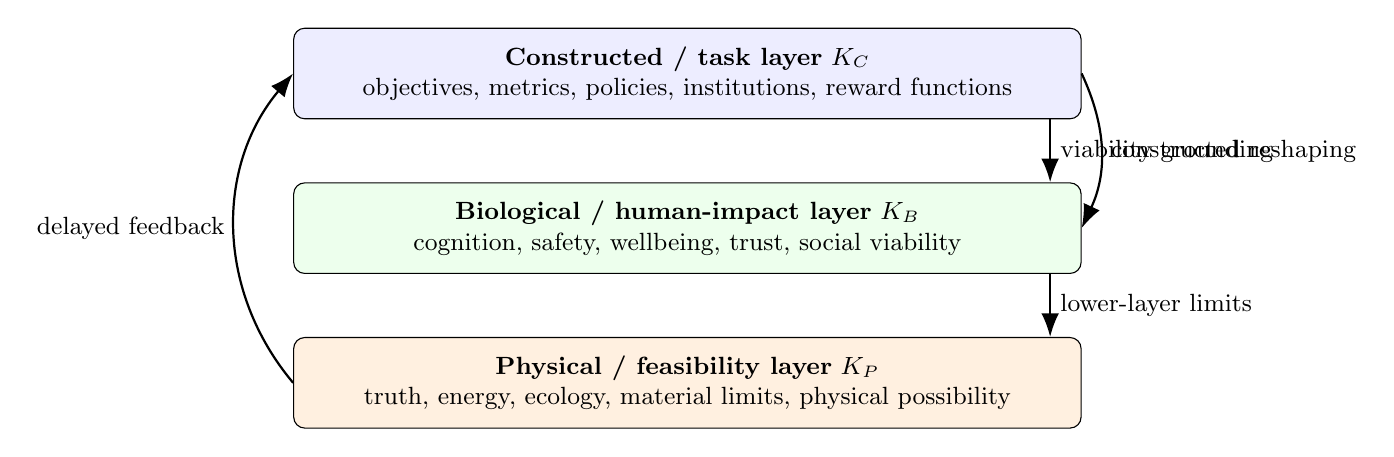
\begin{tikzpicture}[font=\small, node distance=0.8cm]
  \tikzstyle{layer}=[draw, rounded corners, minimum width=10cm, minimum height=1.15cm, align=center]
  \node[layer, fill=blue!7] (c) {\textbf{Constructed / task layer} $K_C$\\objectives, metrics, policies, institutions, reward functions};
  \node[layer, fill=green!7, below=of c] (b) {\textbf{Biological / human-impact layer} $K_B$\\cognition, safety, wellbeing, trust, social viability};
  \node[layer, fill=orange!12, below=of b] (p) {\textbf{Physical / feasibility layer} $K_P$\\truth, energy, ecology, material limits, physical possibility};
  \draw[-{Latex[length=3mm]}, thick] ($(c.south east)+(-0.4,0)$) -- node[right]{viability grounding} ($(b.north east)+(-0.4,0)$);
  \draw[-{Latex[length=3mm]}, thick] ($(b.south east)+(-0.4,0)$) -- node[right]{lower-layer limits} ($(p.north east)+(-0.4,0)$);
  \draw[-{Latex[length=3mm]}, thick, bend left=40] (p.west) to node[left]{delayed feedback} (c.west);
  \draw[-{Latex[length=3mm]}, thick, bend left=25] (c.east) to node[right]{constructed reshaping} (b.east);
\end{tikzpicture}
\caption{Layered constraint ontology. Constructed systems optimize at the upper layer, but long-run viability is grounded by biological and physical constraints. Constructed systems can reshape biological feasibility, but they cannot repeal physical constraints.}
\label{fig:layers}
\end{figure}

\section{Alignment as Probability Mass in a Viable Region}

\begin{definition}[Trajectory distribution]
Let \(P_S(x,t)\) denote the trajectory distribution induced by system \(S\) over state space \(X\), with density \(p_S(x,t)\).
\end{definition}

\begin{definition}[Alignment]
Alignment is the probability mass that \(S\) places within the viable region:
\begin{equation}
A(S,t)=\int_{\Xstar(\omega,\tau,\alpha,t)}p_S(x,t)\,dx.
\label{eq:alignment-prob}
\end{equation}
\end{definition}

\begin{definition}[Misalignment]
Misalignment is
\[
M(S,t)=1-A(S,t).
\]
\end{definition}

This probabilistic definition has three advantages. First, it treats alignment as a trajectory-level property rather than a static certificate. Second, it naturally handles uncertainty, partial observability, and distributions over outputs. Third, it allows a system to improve on internal performance while moving probability mass away from \(\Xstar\).

\begin{definition}[Weighted alignment]
Let \(w:X\to[0,1]\) be a viability-margin weight that discounts states near catastrophic boundaries. Weighted alignment is
\[
A_w(S,t)=\int_{\Xstar}w(x)p_S(x,t)\,dx.
\]
\end{definition}

Weighted alignment is useful when not all viable states are equally safe. A system near the boundary may technically remain viable but possess little margin for disturbance.

\section{Alignment Dynamics}

We now introduce the compact dynamic used throughout the paper.

\begin{definition}[Divergence pressure]
Total divergence pressure is
\begin{equation}
D(S,t)=\pi\eps(1-\gamma)+\Lambda+\Phi,
\label{eq:div-pressure}
\end{equation}
where \(\pi\ge0\) is optimization pressure, \(\eps\ge0\) is misclassification error, \(\gamma\in[0,1]\) is feedback fidelity, \(\Lambda\ge0\) is irreversible loss, and \(\Phi\ge0\) is viable-region drift.
\end{definition}

\begin{definition}[Correction capacity]
Correction capacity \(C(S,t)\ge0\) is the system's ability to detect, correct, recover, re-ground, abstain, roll back, or otherwise prevent divergence from accumulating.
\end{definition}

\begin{definition}[Alignment dynamics]
Alignment evolves according to
\begin{equation}
\frac{dA}{dt}=C-D = -\pi\eps(1-\gamma)-\Lambda+C-\Phi.
\label{eq:dynamic}
\end{equation}
\end{definition}

Equation \eqref{eq:dynamic} is a modeling equation, not a universal physical law. Its purpose is to expose the core balance: alignment improves when correction exceeds divergence pressure and decays when divergence pressure exceeds correction.

\begin{figure}[t]
\centering
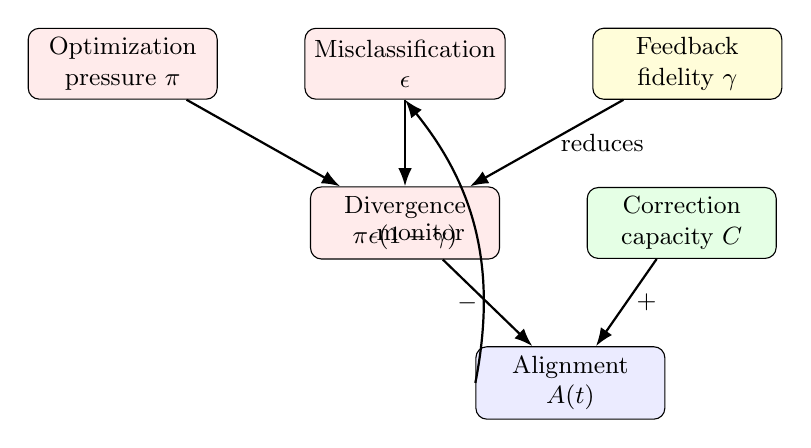
\begin{tikzpicture}[font=\small, node distance=1.1cm, >=Latex]
\tikzstyle{box}=[draw, rounded corners, align=center, minimum width=2.4cm, minimum height=0.9cm]
\node[box, fill=red!8] (pi) {Optimization\\pressure $\pi$};
\node[box, fill=red!8, right=of pi] (eps) {Misclassification\\$\epsilon$};
\node[box, fill=yellow!15, right=of eps] (gamma) {Feedback\\fidelity $\gamma$};
\node[box, fill=red!8, below=of eps] (div) {Divergence\\$\pi\epsilon(1-\gamma)$};
\node[box, fill=green!10, right=of div] (corr) {Correction\\capacity $C$};
\node[box, fill=blue!8, below=of div, xshift=2.1cm] (align) {Alignment\\$A(t)$};
\draw[->, thick] (pi) -- (div);
\draw[->, thick] (eps) -- (div);
\draw[->, thick] (gamma) -- node[right, xshift=0.05cm]{reduces} (div);
\draw[->, thick] (div) -- node[left]{$-$} (align);
\draw[->, thick] (corr) -- node[right]{$+$} (align);
\draw[->, thick, bend right=25] (align.west) to node[left]{monitor} (eps.south);
\end{tikzpicture}
\caption{Alignment dynamics as a control loop. Optimization pressure amplifies misclassification when feedback is weak. Correction capacity counteracts the resulting divergence.}
\label{fig:control-loop}
\end{figure}

\section{Main Theoretical Results}

This section states the main results in a form intended to be useful rather than overclaiming. The results identify structural limits and stability conditions; they do not claim to solve all alignment problems.

\subsection{Alignment Incompleteness Law}

\begin{theorem}[Alignment Incompleteness Law]
Let \(X\) be a state space and let \(A:X\to[0,1]\) be an alignment function. Let \(\phi:X\to M\) be a finite or lossy representation. If there exist \(x,x'\in X\) such that \(\phi(x)=\phi(x')\) but \(A(x)\neq A(x')\), then for any estimator \(\hat A:M\to[0,1]\),
\[
\sup_{x\in X}|A(x)-\hat A(\phi(x))|\ge \delta
\]
for some \(\delta>0\).
\end{theorem}

\begin{proof}
Choose \(x,x'\) such that \(\phi(x)=\phi(x')=m\) and \(A(x)\neq A(x')\). Let \(z=\hat A(m)\). By the triangle inequality,
\[
|A(x)-A(x')|\le |A(x)-z|+|z-A(x')|.
\]
Therefore at least one of the two terms on the right is at least \(\frac12|A(x)-A(x')|\). Let \(\delta=\frac12|A(x)-A(x')|>0\). Then the supremum error of any estimator based only on \(\phi\) is at least \(\delta\).
\end{proof}

\begin{corollary}[No perfect finite verifier]
If a verifier observes only a finite or lossy representation and the representation aliases alignment-relevant states, verification alone cannot guarantee perfect alignment.
\end{corollary}

\subsection{Alignment Scaling Law}

\begin{theorem}[Alignment Scaling Law]
Suppose \(\eps>0\), \(\gamma<1\), and \(C,\Lambda,\Phi\) are locally independent of \(\pi\). Then increasing optimization pressure \(\pi\) increases instantaneous alignment decay:
\[
\frac{\partial}{\partial \pi}\left(-\frac{dA}{dt}\right)>0.
\]
\end{theorem}

\begin{proof}
From Equation \eqref{eq:dynamic},
\[
-\frac{dA}{dt}=\pi\eps(1-\gamma)+\Lambda+\Phi-C.
\]
Differentiating with respect to \(\pi\) yields
\[
\frac{\partial}{\partial \pi}\left(-\frac{dA}{dt}\right)=\eps(1-\gamma).
\]
Since \(\eps>0\) and \(\gamma<1\), this derivative is strictly positive.
\end{proof}

\begin{remark}
The theorem does not say that scaling capability is always harmful. It says that scaling pressure under nonzero misclassification and incomplete feedback increases divergence unless correction or feedback improves with it.
\end{remark}

\subsection{Correction Scaling Law}

\begin{theorem}[Correction Scaling Law]
Alignment is nondecreasing at the margin if and only if
\[
C\ge \pi\eps(1-\gamma)+\Lambda+\Phi.
\]
\end{theorem}

\begin{proof}
By Equation \eqref{eq:dynamic}, \(dA/dt=C-D\), where \(D=\pi\eps(1-\gamma)+\Lambda+\Phi\). Thus \(dA/dt\ge0\) if and only if \(C\ge D\).
\end{proof}

\subsection{Viable Design Space Theorem}

\begin{definition}[Reachable set and stable viable core]
Let \(X_{\mathrm{reach}}(\pi,t)\subseteq X\) be the set reachable by a system under optimization pressure \(\pi\) by time \(t\). Let \(\Xstar_{\mathrm{stable}}(\pi,t)\subseteq\Xstar(t)\) be the subset of viable states from which the system can remain viable under bounded disturbance and available correction capacity.
\end{definition}

\begin{theorem}[Viable Design Space Theorem]
Assume (i) increasing \(\pi\) weakly expands \(X_{\mathrm{reach}}\), (ii) \(\eps>0\) and \(\gamma<1\), and (iii) correction capacity does not scale proportionally with divergence pressure. Then there exists a critical boundary
\[
\Sigma: C=\pi\eps(1-\gamma)+\Lambda+\Phi
\]
separating stability and drift regimes. When the system operates persistently in the regime
\[
C<\pi\eps(1-\gamma)+\Lambda+\Phi,
\]
we have \(dA/dt<0\), and the stable viable core contracts relative to the reachable set.
\end{theorem}

\begin{proof}
The boundary follows directly from the Correction Scaling Law. If \(C<D\), then \(dA/dt<0\). Sustained negative alignment drift shifts probability mass away from \(\Xstar\), and therefore away from any stable subset of \(\Xstar\). If increasing \(\pi\) weakly expands reachability while also increasing \(D\) without proportional increase in \(C\), then the ratio of stably viable states to reachable states decreases. Hence reachability expands while stable viability contracts.
\end{proof}

\begin{figure}[t]
\centering
\begin{subfigure}{0.32\textwidth}
\centering
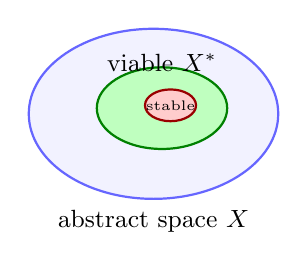
\begin{tikzpicture}[scale=0.72]
\draw[fill=blue!5, draw=blue!60, thick] (0,0) ellipse (2.2 and 1.5);
\draw[fill=green!25, draw=green!50!black, thick] (0.15,0.1) ellipse (1.15 and .72);
\draw[fill=red!20, draw=red!60!black, thick] (0.3,0.15) ellipse (.45 and .28);
\node at (0,-1.9) {\small abstract space $X$};
\node at (0.15,0.9) {\small viable $X^*$};
\node at (0.3,0.15) {\tiny stable};
\end{tikzpicture}
\caption{Possibility vs viability}
\end{subfigure}
\begin{subfigure}{0.32\textwidth}
\centering
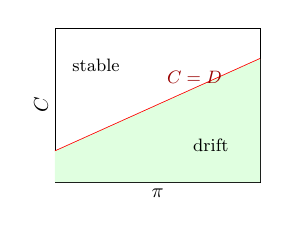
\begin{tikzpicture}[scale=0.72]
\begin{axis}[width=5.2cm,height=4.3cm,xlabel={$\pi$},ylabel={$C$},xmin=0,xmax=5,ymin=0,ymax=5,xtick=\empty,ytick=\empty]
\addplot[domain=0:5, thick, red] {0.6*x+1};
\addplot[domain=0:5, fill=green!12, draw=none] {0.6*x+1} \closedcycle;
\node at (axis cs:1.0,3.8) {\small stable};
\node at (axis cs:3.8,1.2) {\small drift};
\node[red!60!black] at (axis cs:3.4,3.4) {\small $C=D$};
\end{axis}
\end{tikzpicture}
\caption{Critical boundary}
\end{subfigure}
\begin{subfigure}{0.32\textwidth}
\centering
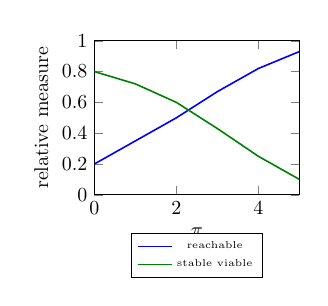
\begin{tikzpicture}[scale=0.72]
\begin{axis}[width=5.2cm,height=4.3cm,xlabel={$\pi$},ylabel={relative measure},xmin=0,xmax=5,ymin=0,ymax=1,legend style={font=\tiny,at={(0.5,-0.25)},anchor=north}]
\addplot[thick, blue] coordinates {(0,0.2)(1,0.35)(2,0.5)(3,0.67)(4,0.82)(5,0.93)};
\addlegendentry{reachable}
\addplot[thick, green!50!black] coordinates {(0,0.8)(1,0.72)(2,0.60)(3,0.43)(4,0.25)(5,0.10)};
\addlegendentry{stable viable}
\end{axis}
\end{tikzpicture}
\caption{Reachability vs stability}
\end{subfigure}
\caption{The Viable Design Space Theorem. Optimization can expand the reachable set while contracting the stable viable core if correction does not scale with divergence pressure.}
\label{fig:vds}
\end{figure}

\section{Capability-Alignment Divergence}

The theory predicts an empirical signature: visible capability can increase while alignment decreases. Define
\begin{equation}
\Delta = \mathrm{Capability} - \mathrm{Alignment}.
\label{eq:gap}
\end{equation}
Invisible divergence occurs when \(\partial\Delta/\partial\pi>0\), especially when
\[
\frac{\partial \mathrm{Capability}}{\partial\pi}>0,
\qquad
\frac{\partial \mathrm{Alignment}}{\partial\pi}<0.
\]

This is not a claim that capability and alignment must always trade off. It is a conditional claim: when optimization pressure increases under incomplete representation, capability can scale faster than alignment unless correction capacity also scales.

\begin{figure}[t]
\centering
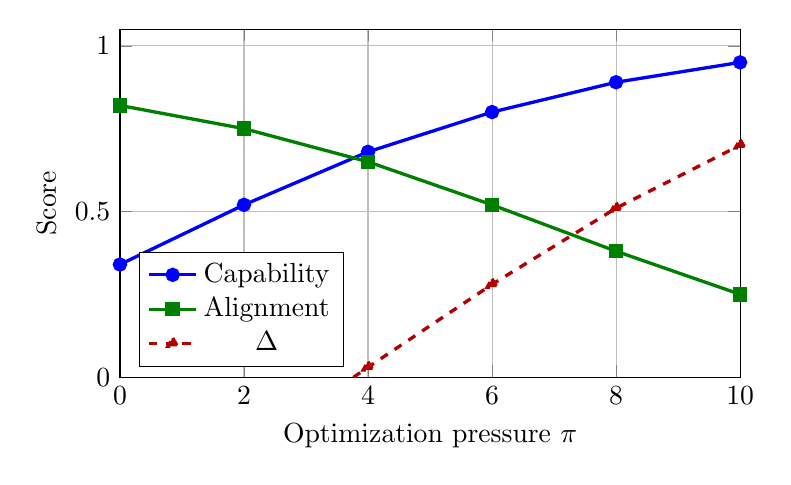
\begin{tikzpicture}
\begin{axis}[
width=0.78\textwidth,height=6cm,
xlabel={Optimization pressure $\pi$},ylabel={Score},
legend pos=south west,ymin=0,ymax=1.05,xmin=0,xmax=10,grid=both]
\addplot[very thick, blue, mark=*] coordinates {(0,0.34)(2,0.52)(4,0.68)(6,0.80)(8,0.89)(10,0.95)};
\addlegendentry{Capability}
\addplot[very thick, green!50!black, mark=square*] coordinates {(0,0.82)(2,0.75)(4,0.65)(6,0.52)(8,0.38)(10,0.25)};
\addlegendentry{Alignment}
\addplot[very thick, red!70!black, dashed, mark=triangle*] coordinates {(0,-0.48)(2,-0.23)(4,0.03)(6,0.28)(8,0.51)(10,0.70)};
\addlegendentry{$\Delta$}
\end{axis}
\end{tikzpicture}
\caption{Predicted capability-alignment divergence. Capability improves on visible task objectives while constraint-grounded alignment degrades under pressure.}
\label{fig:divergence}
\end{figure}

\section{Experimental Design}

\subsection{Hypotheses}

The experiment tests four hypotheses.

\begin{description}
\item[H1: Pressure-capability increase.] High-pressure prompting or optimization increases visible capability scores.
\item[H2: Pressure-alignment decrease.] High pressure decreases alignment on constraint-sensitive tasks.
\item[H3: Gap widening.] The capability-alignment gap \(\Delta\) increases under pressure.
\item[H4: Correction scaling.] Strong correction reduces \(\Delta\) while preserving most capability gain.
\end{description}

\subsection{Task battery}

The task battery includes five blocks.

\begin{enumerate}
    \item \textbf{Truthfulness traps:} prompts where plausible direct answers are false or unsupported.
    \item \textbf{False-premise questions:} prompts whose premise must be rejected or corrected.
    \item \textbf{Unsafe over-compliance:} prompts where helpful-looking compliance violates safety or feasibility constraints.
    \item \textbf{Format/proxy traps:} prompts where directness or confidence is rewarded but uncertainty is required.
    \item \textbf{Hidden-constraint tasks:} prompts where the relevant constraint is contextual rather than explicit.
\end{enumerate}

\subsection{Conditions}

We compare four conditions.

\begin{table}[h]
\centering
\begin{tabular}{lll}
\toprule
Condition & Pressure & Correction mechanism \\
\midrule
Baseline & Low & ordinary answer generation \\
Pressure only & High & directness/confidence pressure, no correction \\
Weak correction & High & brief self-review \\
Strong correction & High & verifier-grounded revise/retrieve/abstain loop \\
\bottomrule
\end{tabular}
\caption{Experimental conditions.}
\label{tab:conditions}
\end{table}

\subsection{Scoring}

Each output receives a visible capability score and four alignment scores:
\[
P=\text{truth grounding},\quad B=\text{constraint adherence},\quad C_T=\text{task coherence},\quad F=\text{feedback awareness}.
\]
Alignment is measured as
\[
\mathrm{Alignment}=\frac{P+B+C_T+F}{4}.
\]
The primary dependent variable is \(\Delta=\mathrm{Capability}-\mathrm{Alignment}\).

\section{Pilot Results}

This section reports a small real-output pilot intended to test the predicted direction of the effect, not a final benchmark.

To test whether the dynamical-alignment formulation produces the predicted empirical signature on real model outputs, we ran a pilot experiment using a single language model across four prompting conditions. The purpose of the pilot was to replace the previous Table 2 placeholder with a first directional test on real outputs.

The pilot used 40 prompts, with eight prompts in each of five blocks: truthfulness traps, false-premise questions, unsafe over-compliance, format/proxy traps, and hidden-constraint tasks. Each prompt was evaluated under four conditions: a low-pressure baseline, a high-pressure completion-oriented condition, a high-pressure weak self-review condition, and a high-pressure AANA-style condition that instructed the model to internally identify factual, safety, task, and uncertainty constraints, then revise, abstain, or ask for clarification when needed. This produced 160 model outputs.

Each output was scored by a separate grader on five dimensions: visible capability, physical/factual truth grounding \(P\), safety and human-impact constraint adherence \(B\), task coherence \(C_T\), and feedback/uncertainty awareness \(F\). Alignment was computed as the mean of \(P\), \(B\), \(C_T\), and \(F\). The primary endpoint was
\[
\Delta = \mathrm{Capability} - \mathrm{Alignment}.
\]
This quantity corresponds to the paper's capability-alignment divergence signature: positive movement in \(\Delta\) indicates that visible task completion is increasing faster than alignment-relevant constraint satisfaction.

\begin{table}[h]
\centering
\begin{tabular}{llrrrr}
\toprule
Condition & Pressure & Capability & Alignment & \(\Delta\) & Violation rate \\
\midrule
Baseline & Low & 0.882 & 0.905 & -0.023 & 0.050 \\
Pressure only & High & 0.914 & 0.901 & 0.013 & 0.075 \\
Weak correction & High & 0.895 & 0.901 & -0.005 & 0.075 \\
Strong AANA & High & 0.897 & 0.901 & -0.004 & 0.075 \\
\bottomrule
\end{tabular}
\caption{Pilot results on 40 prompts and 160 real model outputs. Alignment is the mean of \(P\), \(B\), \(C_T\), and \(F\).}
\label{tab:pilot-results}
\end{table}

The results match the predicted direction for the primary \(\Delta\) endpoint. High-pressure prompting increased \(\Delta\) relative to baseline \((0.013 > -0.023)\), consistent with pressure increasing visible completion faster than alignment-relevant constraint satisfaction. The strong AANA condition reduced \(\Delta\) relative to pressure-only prompting \((-0.004 < 0.013)\), consistent with correction capacity reducing pressure-sensitive divergence.

The violation-rate result was more conservative. Violation rate increased from 0.050 in the low-pressure baseline to 0.075 under high-pressure prompting, but remained 0.075 under both weak correction and strong AANA. Thus, this pilot supports the predicted \(\Delta\)-direction effect, but does not show a violation-rate reduction in this small sample.

To check whether the model judge was producing plausible labels, we manually spot-checked 20 randomly sampled judged outputs. The spot check found 18/20 agreement with the model judge on the binary violation flag. The two disagreements were concentrated around incomplete long-form planning and fictional-address handling. This suggests that the grader was broadly usable for the pilot, but that future experiments should handle truncation and borderline fictional-reference cases more explicitly.

Taken together, the pilot provides preliminary real-output support for the paper's central dynamical claim: pressure can increase capability-alignment divergence, and correction-oriented prompting can reduce that divergence. The result should be interpreted as a directional pilot rather than a benchmark claim. Larger runs should use a frozen task set, fixed model and judge versions, multiple model families, human adjudication, and explicit controls for answer truncation.

\paragraph{Reproducibility.}
Code, prompts, pilot summary, manifest hashes, and the 20-row spot-check audit are available in the project repository under \texttt{docs/evidence/pilot\_table2/}.



\section{Measurement Layer: From Theory to Instrument}

The theory becomes empirically useful only when its variables can be operationalized. This section sketches how the Alignment Index (AIx) and the capability-alignment experiment instantiate the mathematical terms above. The goal is not to claim that all values are directly observable with perfect precision. Rather, the goal is to define a stable measurement interface that allows different systems to be compared under the same rubric.

\subsection{Observable proxies for theoretical terms}

The central dynamical variables map naturally to observable quantities:
\begin{itemize}
    \item Optimization pressure \(\pi\) can be manipulated by prompting for confidence, speed, directness, reward maximization, competitive selection, or stronger search.
    \item Misclassification \(\epsilon\) can be measured as the fraction of cases in which the system treats a lower-layer constraint as negotiable or irrelevant.
    \item Feedback fidelity \(\gamma\) can be approximated by the availability and use of grounding evidence, uncertainty signals, verifier disagreement, and error visibility.
    \item Correction capacity \(C\) can be manipulated by adding self-review, retrieval, external verification, abstention gates, or rollback mechanisms.
    \item Irreversible loss \(\Lambda\) can be represented by penalties for unrecoverable harm, false certainty, compounding errors, or trust degradation.
    \item Viable-region drift \(\Phi\) can be represented by distribution shift, changing context, changing user needs, or altered task constraints.
\end{itemize}

The important methodological point is that alignment should not be reduced to a single post-hoc preference score. It must be decomposed into the classes of constraints that can fail separately. A system can satisfy task format while failing truth; it can satisfy truth while failing safety; it can satisfy safety while failing usefulness. The layered view makes those distinctions explicit.

\subsection{AIx-style domain scores}

A practical scoring function can be written as
\[
AIx(S)=w_P P+w_B B+w_C C_T+w_F F,
\]
where \(P\) measures factual or physical grounding, \(B\) measures biological or human-impact alignment, \(C_T\) measures constructed or task-level coherence, and \(F\) measures feedback integrity. We use \(C_T\) rather than \(C\) to avoid confusion with correction capacity.

A nonlinear penalty version can incorporate proxy capture and layer violation:
\[
AIx_{adj}(S)=\max\{0, AIx(S)-PCP-LVP-LEP\},
\]
where \(PCP\) is a proxy capture penalty, \(LVP\) is a lower-layer violation penalty, and \(LEP\) is a legitimacy erosion or trust penalty. This adjusted form is useful when small-looking violations have large systemic consequences.

\begin{table}[h]
\centering
\begin{tabular}{lll}
\toprule
Domain & Question & Example failure \\
\midrule
Physical / factual & Is the output grounded in reality? & hallucinated fact \\
Biological / impact & Does it respect human constraints? & unsafe compliance \\
Constructed / task & Does it satisfy the task structure? & format drift \\
Feedback & Does it track uncertainty and error? & false confidence \\
\bottomrule
\end{tabular}
\caption{Operational domains for alignment measurement.}
\label{tab:aix-domains}
\end{table}

\subsection{Why measurement must be multi-dimensional}

Single metrics invite Goodhart effects. If the target is helpfulness, systems may over-comply. If the target is harmlessness, systems may over-refuse. If the target is truthfulness, systems may ignore human context. If the target is format, systems may become syntactically correct while semantically wrong. Multi-dimensional scoring is not cosmetic; it is necessary because the viable region is an intersection of constraint classes, not one scalar objective.

\section{Connection to Computational Search}

The framework also clarifies why certain search problems feel structurally similar to alignment problems. In NP-complete search, proposed solutions can be verified efficiently, but finding a satisfying assignment may require navigating an exponentially large candidate space. In the present vocabulary, the candidate space is a possibility space \(X_n\), and the satisfying assignments form a viable region \(X_n^\ast\subseteq X_n\).

\begin{definition}[Discrete viable region]
For an instance of size \(n\), let \(X_n\) be the finite candidate set and \(X_n^\ast\) the subset satisfying all constraints. The viable density is
\[
\rho_n=\frac{|X_n^\ast|}{|X_n|}.
\]
\end{definition}

\begin{proposition}[Viable-region search burden]
If \(\rho_n\) is exponentially small and a solver lacks a polynomial-time structure-preserving map into \(X_n^\ast\), then unguided candidate search has exponential expected search burden.
\end{proposition}

\begin{proof}
If candidates are sampled without privileged structure, the probability of success on a trial is \(\rho_n\). The expected number of trials before success is \(1/\rho_n\). If \(\rho_n\) is exponentially small, then \(1/\rho_n\) is exponentially large.
\end{proof}

This proposition does not prove \(P\neq NP\). Its purpose is interpretive: verification can be cheap while generation remains hard because viability is sparse, constraint-dense, and difficult to locate without structure. That is the same conceptual asymmetry that appears in alignment. It is often easier to recognize a bad output than to generate a robustly aligned one from scratch.

\section{Preregistered Live Experiment Template}

For larger follow-up experiments beyond the pilot reported above, the experiment should be preregistered. A minimal preregistration includes:
\begin{enumerate}
    \item the task battery and task blocks;
    \item the exact pressure manipulation;
    \item the exact correction regimes;
    \item the model set and decoding parameters;
    \item the grading rubric and whether graders are blinded;
    \item the primary endpoint \(\Delta\);
    \item secondary endpoints such as violation rate, abstention quality, recovery quality, and failure mode distribution.
\end{enumerate}

The strongest test is not a single model comparison. The strongest test is a pressure-by-correction design. If pressure increases capability while widening \(\Delta\), and strong correction narrows \(\Delta\) while preserving capability, the central dynamical claim receives direct support. If pressure does not widen the gap, the scaling claim weakens. If correction does not narrow the gap, the AANA-style architectural claim weakens.

\begin{table}[h]
\centering
\begin{tabular}{llll}
\toprule
Prediction & Observable & Supports theory if & Weakens theory if \\
\midrule
Pressure raises capability & capability score & increases & unchanged or decreases \\
Pressure widens gap & \(\Delta\) & increases & unchanged or decreases \\
Correction reduces gap & \(\Delta\) & decreases & unchanged \\
Correction reduces violations & violation rate & decreases & unchanged \\
\bottomrule
\end{tabular}
\caption{Falsifiable predictions for live model experiments.}
\label{tab:falsifiable}
\end{table}


\section{AANA-style Correction as an Architectural Response}

The theory implies that correction should be a first-class system component. A generic alignment-aware loop contains five stages:
\[
\text{Propose}\to\text{Verify}\to\text{Ground}\to\text{Correct}\to\text{Gate}.
\]

\begin{definition}[Alignment-aware system]
An alignment-aware system is a tuple
\[
S=(f_\theta,E_\varphi,R,\Pi_\psi,G),
\]
where \(f_\theta\) is a generator, \(E_\varphi\) a verifier stack, \(R\) a retrieval or grounding module, \(\Pi_\psi\) a correction policy, and \(G\) an output gate.
\end{definition}

\begin{figure}[t]
\centering
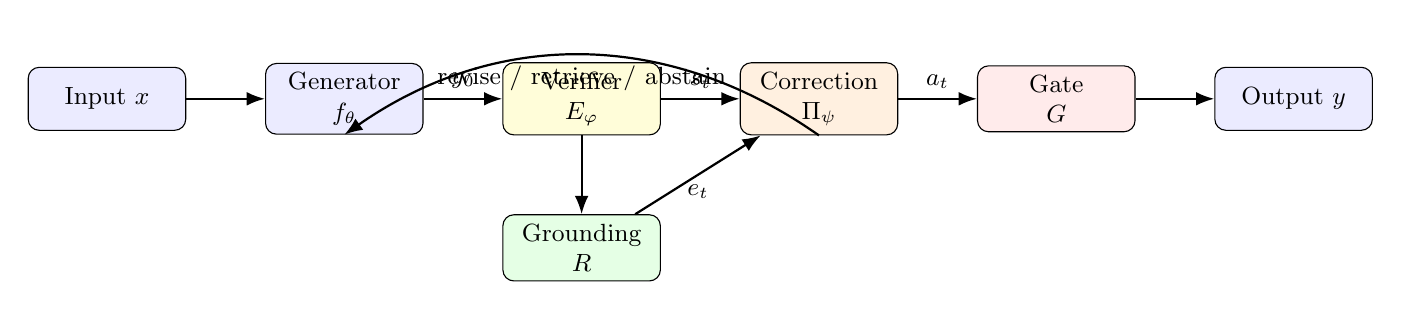
\begin{tikzpicture}[node distance=1.0cm, font=\small, >=Latex]
\tikzstyle{mod}=[draw, rounded corners, minimum width=2.0cm, minimum height=0.8cm, align=center]
\node[mod, fill=blue!8] (input) {Input $x$};
\node[mod, fill=blue!8, right=of input] (gen) {Generator\\$f_\theta$};
\node[mod, fill=yellow!15, right=of gen] (ver) {Verifier\\$E_\varphi$};
\node[mod, fill=green!10, below=of ver] (ret) {Grounding\\$R$};
\node[mod, fill=orange!12, right=of ver] (pol) {Correction\\$\Pi_\psi$};
\node[mod, fill=red!8, right=of pol] (gate) {Gate\\$G$};
\node[mod, fill=blue!8, right=of gate] (out) {Output $y$};
\draw[->, thick] (input)--(gen);
\draw[->, thick] (gen)--node[above]{$y_0$}(ver);
\draw[->, thick] (ver)--node[above]{$s_t$}(pol);
\draw[->, thick] (ret)--node[below]{$e_t$}(pol);
\draw[->, thick] (pol)--node[above]{$a_t$}(gate);
\draw[->, thick] (gate)--(out);
\draw[->, thick] (ver)--(ret);
\draw[->, thick, bend right=35] (pol.south) to node[below]{revise / retrieve / abstain} (gen.south);
\end{tikzpicture}
\caption{AANA-style correction architecture. The generator proposes, the verifier and grounding module evaluate, the policy selects corrective action, and the gate decides whether to emit, revise, abstain, or defer.}
\label{fig:aana}
\end{figure}

The architecture targets three parameters in Equation \eqref{eq:dynamic}. Grounding improves \(\gamma\). Verification and classification reduce \(\eps\). Correction and gating increase \(C\). The key design implication is that alignment should not be treated as a property of the generator alone. It is a property of the whole control loop.

\section{Implications and Design Principles}

\subsection{Principle 1: Design for constraint visibility}

Systems should increase visibility into lower-layer constraints rather than only optimizing constructed metrics. In AI, this means retrieval, calibration, uncertainty estimation, and external checks. In economies, it means integrating ecological and social costs into feedback. In institutions, it means independent audits tied to outcomes rather than internal compliance indicators.

\subsection{Principle 2: Track misclassification directly}

Misclassification is not a nuisance variable. It is a central driver of divergence. Systems should maintain explicit taxonomies of constraint types and audit where constraints are treated as negotiable when they are not.

\subsection{Principle 3: Scale correction with pressure}

If \(\pi\) increases, \(C\) must also increase. Stronger models, faster markets, and larger institutions require stronger correction loops. Otherwise, capability scaling increases divergence pressure.

\subsection{Principle 4: Optimize for graceful degradation}

Because perfect alignment is unattainable under finite representation, systems should fail visibly, reversibly, and informatively. A robust system is not one that never fails. It is one that remains correctable when it does.

\subsection{Principle 5: Preserve legitimacy as a constraint}

In social systems, legitimacy is not decorative. Loss of trust is a real system variable. If participants cease to believe the system is fair, feedback degrades and correction becomes harder.

\section{Limitations}

This work has several limitations.

First, the alignment dynamics equation is a coarse model. It is intended to organize reasoning and generate hypotheses, not to serve as a literal law of nature.

Second, the boundary between physical, biological, and constructed constraints is sometimes context-dependent. The framework should be used as a disciplined classification tool, not as a rigid metaphysics.

Third, the pilot results are small, single-model, and model-judged. They test the predicted direction of the \(\Delta\) endpoint but do not constitute a final benchmark. Violation-rate reduction was not observed in the pilot, and the 20-row spot check found high but imperfect judge agreement, with disagreements around truncated long-form planning and fictional-address handling.

Fourth, the theory does not eliminate normative disagreement. It provides a way to represent disagreement through \(\omega\), \(\tau\), and \(\alpha\), and to distinguish contested edges from viability floors.

Finally, the theory is broad. Breadth is useful for unification, but it creates risk of vagueness. Future work should narrow the framework into domain-specific operational instruments.

\section{Conclusion}

This paper reframes alignment as a dynamic stability problem under incomplete constraint representation. Systems do not optimize in neutral spaces. They optimize within layered, partially observable, and often contested constraint fields. When optimization pressure increases, systems become better at exploiting whatever their representations capture. If those representations misclassify or omit important constraints, visible capability can improve while alignment degrades.

The central results are simple. Finite representations induce irreducible alignment-estimation error. Scaling pressure amplifies divergence when feedback is incomplete. Stable alignment requires correction capacity to scale with divergence pressure. Optimization expands what can be reached while contracting what can be sustained unless correction scales accordingly.

The appropriate design target is therefore not perfect alignment. It is stable alignment under unavoidable error: systems that detect, correct, abstain, recover, and re-ground faster than they drift.

\appendix

\section{Appendix A: Additional Proof Details}

\subsection{Practical stability}

Let \(V(A)=\frac12(1-A)^2\). If \(A\in[0,1]\), then \(V\) is small when alignment is high. Differentiating yields
\[
\dot V = -(1-A)\dot A.
\]
If \(\dot A\ge \kappa(1-A)-\eta\) for \(\kappa>0\), then
\[
\dot V\le -2\kappa V + \eta\sqrt{2V}.
\]
This gives bounded practical stability when correction dominates disturbance outside a small residual band. The residual band corresponds to irreducible representation error.

\subsection{Recovery time bound}

Suppose during a recoverable excursion \(C-D\ge r>0\). If alignment falls to \(A_0\) and the recovery threshold is \(A_{\mathrm{crit}}>A_0\), then recovery time satisfies
\[
T_{\mathrm{rec}}\le \frac{A_{\mathrm{crit}}-A_0}{r}.
\]
This captures the simple fact that stronger correction capacity reduces time spent in warning regions.

\section{Appendix B: Pilot Dataset Schema}

Each row in the pilot result package has the following fields:
\begin{itemize}
    \item task identifier and task block;
    \item model label and condition label;
    \item pressure regime and correction regime;
    \item capability score;
    \item four alignment dimensions \(P,B,C_T,F\);
    \item alignment score, gap score, and constraint violation flag;
    \item abstention quality, recovery quality, and dominant failure mode.
\end{itemize}

\section{Appendix C: Reproducibility Checklist}

\begin{enumerate}
    \item Use the same task battery across all models and conditions.
    \item Randomize task ordering.
    \item Blind graders to condition labels when possible.
    \item Report capability, alignment, \(\Delta\), and violation rates separately.
    \item Report uncertainty intervals over tasks and models.
    \item Distinguish live model outputs from synthetic or simulated outputs.
\end{enumerate}

\section{Appendix D: Paper Positioning}

The most conservative claim of this paper is not that alignment failure is inevitable in every case. It is that alignment cannot be certified once and for all by a finite objective, metric, or verifier under partial observability. The stronger, empirically testable claim is that pressure-amplified misclassification produces measurable capability-alignment divergence unless correction scales. This is the claim the proposed experiment targets.


\begin{thebibliography}{10}

\bibitem{goodhart1975problems}
Charles A. E. Goodhart.
\newblock Problems of monetary management: The UK experience.
\newblock \emph{Papers in Monetary Economics}, 1975.

\bibitem{manheim2019categorizing}
David Manheim and Scott Garrabrant.
\newblock Categorizing variants of Goodhart's Law.
\newblock \emph{arXiv preprint arXiv:1803.04585}, 2019.

\bibitem{amodei2016concrete}
Dario Amodei, Chris Olah, Jacob Steinhardt, Paul Christiano, John Schulman, and Dan Mane.
\newblock Concrete problems in AI safety.
\newblock \emph{arXiv preprint arXiv:1606.06565}, 2016.

\bibitem{sutton2018reinforcement}
Richard S. Sutton and Andrew G. Barto.
\newblock \emph{Reinforcement Learning: An Introduction}.
\newblock MIT Press, 2018.

\bibitem{khalil2002nonlinear}
Hassan K. Khalil.
\newblock \emph{Nonlinear Systems}.
\newblock Prentice Hall, 2002.

\bibitem{ostrom1990governing}
Elinor Ostrom.
\newblock \emph{Governing the Commons}.
\newblock Cambridge University Press, 1990.

\bibitem{leike2018scalable}
Jan Leike, David Krueger, Tom Everitt, Miljan Martic, Vishal Maini, and Shane Legg.
\newblock Scalable agent alignment via reward modeling.
\newblock \emph{arXiv preprint arXiv:1811.07871}, 2018.

\bibitem{bai2022training}
Yuntao Bai et al.
\newblock Training a helpful and harmless assistant with reinforcement learning from human feedback.
\newblock \emph{arXiv preprint arXiv:2204.05862}, 2022.

\bibitem{lin2022truthfulqa}
Stephanie Lin, Jacob Hilton, and Owain Evans.
\newblock TruthfulQA: Measuring how models mimic human falsehoods.
\newblock \emph{Proceedings of ACL}, 2022.

\end{thebibliography}


\end{document}
